\documentclass[conference]{IEEEtran}
\IEEEoverridecommandlockouts
% The preceding line is only needed to identify funding in the first footnote. If that is unneeded, please comment it out.
\usepackage{cite}
\usepackage{amsmath,amssymb,amsxtra,amsfonts,cancel}
\usepackage{xspace}
\usepackage{algorithmic}
\usepackage{graphicx}
\usepackage{textcomp}
\usepackage{xcolor}
\usepackage{xurl}
\usepackage{todonotes}
\def\BibTeX{{\rm B\kern-.05em{\sc i\kern-.025em b}\kern-.08em
    T\kern-.1667em\lower.7ex\hbox{E}\kern-.125emX}}


\newcommand{\powerset}[1]{\ensuremath{2^{#1}}} % power set
\newcommand{\AF}{\ensuremath{\mathcal{F}}\xspace} % Abstract argumentation framework
\newcommand{\F}{\ensuremath{\mathcal{F}}\xspace} % Abstract argumentation framework
\newcommand{\args}{\ensuremath{\mathsf{A}}\xspace} % Set of arguments
\newcommand{\atts}{\ensuremath{\rightarrow}\xspace}
\newcommand{\attackers}[2]{\ensuremath{\mathcal{F}_{#1}(#2)\xspace}} % Attacker set
\newcommand{\AFC}{\ensuremath{\AF=(\args,\atts)}\xspace} % Definition of an abstract argumentation framework
\newcommand{\cA}{\ensuremath{\mathcal{A}}} % some argument
\newcommand{\cB}{\ensuremath{\mathcal{B}}} % some argument
\newcommand{\cC}{\ensuremath{\mathcal{C}}} % some argument
\newcommand{\argin}{\ensuremath{\mathsf{in}}} % argument is in
\newcommand{\argout}{\ensuremath{\mathsf{out}}} % argument is out
\newcommand{\argundec}{\ensuremath{\mathsf{undec}}} % argument is undec

\newcommand{\Given}{\textbf{Given}\xspace}
\newcommand{\decide}{\textbf{decide}\xspace}
\newcommand{\Enumerate}{\textbf{enumerate}\xspace}
\newcommand{\return}{\textbf{return}\xspace}

\newcommand{\af}{AF}

\newcommand{\cf}{\mathbf{cf}}
\newcommand{\ad}{\mathbf{ad}}
\newcommand{\co}{\mathbf{co}}
\newcommand{\pr}{\mathbf{pr}}
\newcommand{\st}{\mathbf{st}}
\newcommand{\sst}{\mathbf{sst}}
\newcommand{\stg}{\mathbf{stg}}
\newcommand{\gr}{\mathbf{gr}}
\newcommand{\id}{\mathbf{id}}

\newcommand{\se}{\mathbf{SE}}
\newcommand{\ee}{\mathbf{EE}}
\newcommand{\dc}{\mathbf{DC}}
\newcommand{\ds}{\mathbf{DS}}
\newcommand{\dyn}{\mathbf{D}}
\newcommand{\ex}{\mathbf{EX}}
\newcommand{\nem}{\mathbf{NE}}






\begin{document}

\title{Encoding Extension-based Problems in Argumentation to QUBO}

\author{\IEEEauthorblockN{1\textsuperscript{st} Marco Baioletti}
\IEEEauthorblockA{\textit{Dipartimento di Matematica e Informatica} \\
\textit{University of Perugia}\\
Perugia, Italy \\
marco.baioletti@unipg.it}
\and
\IEEEauthorblockN{2\textsuperscript{nd} Francesco Santini}
\IEEEauthorblockA{\textit{Dipartimento di Matematica e Informatica} \\
\textit{University of Perugia}\\
Perugia, Italy \\
francesco.santini@unipg.it}
}

\maketitle

\begin{abstract}
We propose an encoding of several NP-complete problems in extension-based Abstract Argumentation into \emph{Quadratic Unconstrained Binary Optimization} problems. The obtained formulation can be then solved by using quantum annealers, as already accomplished in preliminary tests.
\end{abstract}

\begin{IEEEkeywords}
Abstract Argumentation, Quadratic Unconstrained Binary Optimization.
\end{IEEEkeywords}

\section{Introduction}\label{sect:intro}
\emph{Formal Argumentation} can be credited to the pioneering works in logics of Pollock~\cite{pollock92}, Vreeswijk~\cite{vreeswijk92}, and Simari and Loui~\cite{simari92}. The premise is that (non-monotonic) reasoning can be done by creating and assessing arguments, which are made up of several justifications for a claim's validity. Arguments differ from proofs in that they are defeasible, meaning that other arguments may challenge the validity of their conclusions. Therefore, whether a claim can be accepted depends not only on whether an argument supporting it exists, but also on whether potential opposing arguments exist, which can then be contested by attacking arguments, and so on.

The \emph{Abstract Argumentation} theory of Dung~\cite{Dung:1995} provides the foundation for a lot of current argumentation research. An argumentation framework, which is essentially a directed graph with the arguments represented as nodes and the attack relation represented by arrows, is the key idea in this study. An analysis of the question of which set(s) of arguments can be accepted, given such a network, leads to the definition of an argumentation semantics. 
The argumentation is said to be ``abstract'' because arguments have no internal structures and the there is no specification of what an argument or an attack is. Such a graph-language is however enough to represent conflict among information, and it has connections with well-founded semantics of logic programs~\cite{wellfounded}.
On the  other hand, in ``structured argumentation'',  the premises and claim of an argument are made explicit, and the relationship between the premises and claim is formally defined by using logical entailment, for example (see an example in Sect.~\ref{sect:bgarg}).

In regard of Abstract Argumentation, a number of proposals have been made in the literature; in Section~\ref{sect:bgarg} we summarise the background on  some NP-complete problems  that are related to \emph{extensions}, which are sets of arguments that can survive the conflict together and thus represent collectively a reasonable position an autonomous reasoner might take. 


A \emph{Quadratic Unconstrained Binary Optimization} problem~\cite{firstworkqubo} (\emph{QUBO}),  is a mathematical formulation that  encompasses a wide range of critical \emph{Combinatorial Optimization} problems~\cite{survey2,survey1}.  QUBO problems are  NP-complete, and a vast literature is dedicated to approximate solvers  based on heuristics or meta-heuristics, such as  \emph{simulated annealing} approaches (\emph{SA}), \emph{tabu-serch}, \emph{genetic algorithms} or \emph{evolutionary computing}~\cite{survey1}. \emph{Quantum} annealers  and Fujitsu's \emph{digital annealers}\footnote{Fujitsu's digital annealer: \url{https://www.fujitsu.com/global/services/business-services/digital-annealer/}.} can be used to find global minima by using quantum \emph{fluctuations}.  QUBO models are  at the heart of experimentation with quantum computers built by D-Wave Systems.\footnote{D-Wave webiste: \url{https://www.dwavesys.com}.}

In this paper we propose encodings of different Abstract Argumentation problems that are NP-complete problems as well. The  results, here summarised, are new with respect to the pioneer  work in \cite{pricai22}. As a general result, our goal is to deepen  the research line opened there with the purpose to model  and solve a wide range of this kind of reasoning problems, with the help of quantum machines.

\section{Background}\label{sect:background}


\subsection{Argumentation.}\label{sect:bgarg} An \emph{Abstract Argumentation Framework} (\af, for short) \cite{Dung:1995}
is a tuple $\F=(\args,\atts)$ where
\args is a set of arguments and
\atts is a relation $\atts\subseteq \args\times\args$.
For two arguments $a,b\in\args$ the relation $a \atts b$ means that argument $a$ \emph{attacks} argument $b$.
%For $\cA\in\args$ define $\attackers{\F}{\cA}=\{\cB\mid \cB\atts \cA\}$.
An argument $a \in \args$ is \emph{defended} by $S \subseteq \args$ (in $\F$)
if for each $b \in \args$ such that $b \atts a$
there is some $c \in S$ such that $c \atts b$.
%Define $F: 2^{\args} \rightarrow 2^{\args}$ via $F(S)  = \{ \cA\in\args \mid S \text{~defends~} \cA\}$ where a set $S\subseteq\args$ defends an argument $\cA$ if for all arguments $\cB\in \args$, if $\cB\atts \cA$ then there is $\cC\in E$ with $\cC\atts \cB$.
A set $E \subseteq \args$ is \emph{conflict-free} ($\cf$ in \F) if and only if there are no $a,b\in E$ with $a \atts b$.
$E$ is \emph{admissible} ($\ad$ in \F) if and only if it is conflict-free and each $a \in E$ is defended by $E$.
Finally, the range of $E$ in $\F$, i.e., $E^{+}_\F$, collects the same $E$ and the set of arguments attacked by $E$: $E^{+}_\F=E \cup \{a\in\args \mid \exists b\in E: b \atts a\}$.


The \emph{collective acceptability} of  arguments depends on the definition of
different \textit{semantics}~\cite{Dung:1995}.  Semantics determine
sets of jointly acceptable arguments, called \emph{extensions}, by
mapping each \AFC to a set $\sigma(\F) \subseteq \powerset{\args}$, where $\powerset{\args}$ is the  power set of $\args$, and $\sigma$ parametrically stands for any of the considered semantics.
The extensions under complete, preferred, stable,  and semi-stable
semantics are defined as follows.
Given \AFC and a set $E \subseteq \args$, $E \in \co(\F)$ iff $E$ is admissible in $\F$ and if $a \in \args$ is defended by $E$ in $\F$ then $a\in E$;  $E \in \pr(\F)$ iff $E \in \co(\F)$ and there is no $E' \in \co(\F)$ s.t.\ $E' \supset E$; $E \in \sst(\F)$ iff $E \in \co(\F)$ and there is no $E' \in \co(\F)$ s.t.\ $E'^+_\F \supset E^+_\F$; $E \in \st(\F)$ iff $E \in \co(\F)$ and $E^+_\F = \args$,


\begin{figure}[t]
	\centering
	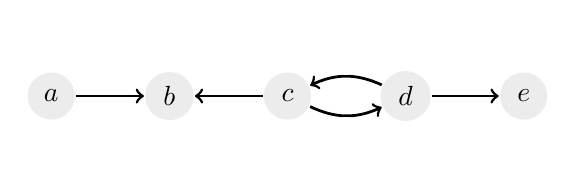
\begin{tikzpicture}[scale=1, transform shape]
		\tikzstyle{every node} = [line width=1pt, shape=circle, fill=gray!15, minimum width=0.6cm]
		\node (a) at (3, 0) {$a$};
		\node (b) at +(0: 4.5) {$b$};
		\node (c) at +(0: 6) {$c$};
		\node (d) at +(0: 7.5) {$d$};
		\node (e) at +(0: 9) {$e$};
		\draw [line width = 1pt, ->] (a) -- (b) node[pos=.5, fill=white, above] {};
		\draw [line width = 1pt, ->] (c) -- (b) node[pos=.5, fill=white, above] {};
		\draw [line width = 1pt, ->] (d) -- (e) node[pos=.5, fill=white, above] {};
		\draw [line width = 1pt, ->] (c)  edge[bend right=25]   node[fill=white, below] {} (d);
		\draw [line width = 1pt, ->] (d) edge[bend right=25] node[fill=white, above] {} (c);
	\end{tikzpicture}
	\vspace{-0.3cm}
	\caption{An example of  WAAF.}\label{fig:argnetex}
\end{figure}


Figure~\ref{fig:argnetex} shows an \af \, with five arguments and five attacks. Given $\F$, the set of complete extensions is $\co(\F) = \{\{a\}, \{a,d\}, \{a, c,e\}\}$, while $\st(\F) = \{\{a,d\}, \{a, c,e\}\}$ is the set of stable extensions, for example. As advanced in Sect.~\ref{sect:intro}, an \AF could represent an abstract view of a structured argumentation: for example, considering Fig.~\ref{fig:argnetex}, we might have that \emph{a:} ``Official reports from rating agencies say the financial crisis dramatically impacted on the overall government budget'' attacks \emph{b:} ``The budget allocated to healthcare for light drugs needs to be increased, because statistics say the number of light drugs users suffering from effects is increasing, and treatments are expensive''.



We  now report  the definition of six well-known decision problems in Abstract Argumentation (yes/no answer).
\emph{Credulous acceptance} $\dc\textit{-}\sigma$: given \AFC and an argument $a \in \args$, is $a$ contained in some $E \in \sigma(\F)$?
Sceptical acceptance $\ds\textit{-}\sigma$: given \AFC and an argument $a \in \args$, is $a$ contained in all $E \in \sigma(\F)$?
\emph{Verification of an extension} $\mathit{\textbf{VER}}\textit{-}\sigma$: given \AFC and a set of arguments $E \subseteq \args$, is $E \in \sigma(\F)$?
\emph{Existence of an extension} $\ex\textit{-}\sigma$: given \AFC, is
$\sigma(\F) \not= \varnothing$?
\emph{Existence of non-empty extension}
$\nem\textit{-}\sigma$: given \AFC, does there exist $E
\not= \varnothing$ such that $E \in \sigma(\F)$?



\begin{table}[t]
	\centering
	\footnotesize
	\begin{tabular}{ccccccc}
		&  Ver-$\sigma$ &  DC-$\sigma$ & DS-$\sigma$ & Ex-$\sigma$ &
		NE-$\sigma$  \\
		Conflict-free & in L & in L & triv.& triv. & in L  \\
		Admissible & in L  & \bf{NP-c} & triv. & triv. &  \bf{NP-c}  \\
		Complete & in L &  \bf{NP-c} & P-c & triv. &  \bf{NP-c}  \\
		Preferred & coNP-c &  \bf{NP-c} & $\prod^{P}_{2}$-c& triv. &  \bf{NP-c} \\
		Semi-stable & coNP-c & $\sum^{P}_{2}$-c & $\prod^{P}_{2}$-c & triv. &  \bf{NP-c}  \\
		Stable & in L &  \bf{NP-c} & coNP-c &  \bf{NP-c} &  \bf{NP-c} \\
	\end{tabular}
	\caption{The complexity of some  problems in Abstract Argumentation; NP-complete problems are highlighted in bold.}
	\label{sec:complexity}
	\vspace{-0.5cm}
\end{table}

In addition, the work in \cite{extenf} presents the task of \emph{extension enforcement}: the goal is to change the attack relationship $\atts$ of a framework $\F=(\args,\atts)$ such that a given set $T \subseteq \args$ becomes (a subset of) an extension under a given semantics $\sigma$. \emph{Strict enforcement} is satisfied if $T$ is a $\sigma$-extension, while in \emph{non-strict enforcement} $T$ is only required to be a subset of a $\sigma$-extension. The complexity is reported in Tab.~\ref{sec:complexity2}.



\begin{table}[t]
	\centering
	\footnotesize
	\begin{tabular}{ccc}
		$\sigma$ &  strict & non-strict  \\
		Admissible & P  & \bf{NP-c}   \\
		Complete & \bf{NP-c} &  \bf{NP-c}  \\
		Preferred & $\sum^{P}_{2}$-c  &  \bf{NP-c}  \\
		Stable &  P & \bf{NP-c}  \\
		Grounded & \bf{NP-c} & \bf{NP-c}
	\end{tabular}
	\caption{The complexity of strict and non-strict extension enforcement.}
	\label{sec:complexity2}
	\vspace{-0.5cm}
\end{table}


\subsection{QUBO}\label{sect:qubo}
\emph{Quadratic Unconstrained Binary Optimization} (\emph{QUBO})~\cite{glover,glover2} is a
form of optimization problems encompassing e.g. SAT/Constraint/(0,1)-ILP, which  recently gained a great popularity because of fast solvers and dedicated computing devices, such as
quantum and digital annealers. 
A QUBO problem is defined in terms of $n$ binary variables $x_1,\dots,x_n$
and a $n\times n$ upper-diagonal matrix $\mathcal{Q}$ and consists in 
minimizing the function $f(x) = \sum_{i=1}^n Q_{i,i} x_i + \sum_{i < j}^n Q_{i,j} x_i x_j$.
The diagonal terms $Q_{i,i}$ are the linear coefficients and the non-zero off-diagonal terms $Q_{i,j}$
are the quadratic coefficients. This can be expressed more concisely as $\min_{x \in \{0,1\}^n} x^T Q x$, where $x^T$ denotes the transpose of the vector $x$. The formulation of a discrete constrained optimization problem as QUBO requires
the following steps {\bf i)}  find a binary representation for the solutions {\bf ii)}  define a penalization function, which penalizes unfeasible solutions (i.e., violating a constraint).

\section{Encoding of problems}\label{sect:encoding}
In \cite{pricai22} we proposed an encoding of two well-known NP-complete problems in Abstract Argumentation (both considering the complete semantics, see Sect.~\ref{sect:bgarg}) as QUBO problems, which share the same complexity: the encoded problems are  
$\dc\textit{-}\sigma$ and
%$\mathit{\textbf{Exists}}\textit{-}\sigma$, and 
$\mathit{\textbf{Exists}}\textit{-}\sigma^{\neg\varnothing}$, 
while the considered semantics was only $\co$.  
Moreover, in \cite{pricai22} we solved this problem on some frameworks directly  implementing them by using the D-Wave Ocean SDK. We both used a simulated annealing algorithm and a real quantum annelaer provided by the \emph{LeapTM Quantum Cloud Service}.\footnote{D-Wave Ocean SDK: \url{https://github.com/dwavesystems/dwave-ocean-sdk}.}

With respect to \cite{pricai22}, by continuing on this research line, we have extended the encoding to all classical NP-complete problems in Tab.~\ref{sec:complexity}.
%with Harper++ and AFGCN. 




\section{Conclusion}\label{sec:conclusion}
In \cite{pricai22} we have used the Ocean SDK\footnote{D-Wave Ocean SDK: \url{https://github.com/dwavesystems/dwave-ocean-sdk}.} to build the encoding in Python and then to solve it on a real D-Wave quantum machine; the logical graph representing the QUBO  model needs to be first embedded into the physical graph of D-Wave's hardware.

\bibliographystyle{IEEEtran}
\bibliography{main}

\end{document}
